\section{Analog-to-Digital Data Converter}
\subsection{Necessary Specifications}
\label{sec:ADC_Parameters}
\indent The BeagleBone Black microcontroller features an on board 12-bit analog-to-digital converter (ADC). From literature, the lowest acceptable
effective resolution that an ADC being used for SHM may have is 16 bits\cite{Cunha_Caetano} \cite{JangSWMWSS}. It was determined that the need for an
external ADC was present. The parameters of the external ADC needed were as follows:
\begin{itemize}
\item High Resolution
\item Appropriate Sampling Frequency
\item Low Power Consumption 
\item Support for Multiple Input Channels
\item Communicate via Serial Interface
\end{itemize}
\subsubsection{Resolution}
\label{sec:adc_res}
\indent Resolution is defined as the number of bits that an analog signal is mapped to after being converted\cite{MusaJouaneh:2013}. Using the chart in
Figure \ref{fig:ADC_Comp_Chart}, it was evident that in order to achieve high resolution data that a Delta-Sigma ($\Delta\Sigma$) ADC needed to be used.\\
\indent As previously stated, the minimum resolution required for this sensor package was 16-bits. The voltage resolution can be found using Equation
\ref{eqn:Resolution}:
\begin{equation}
\label{eqn:Resolution}
V_{Res} = \frac{V_{Range}}{2^{n}}
\end{equation}
Assuming $V_{Range}=3.3V$, $n=16$ bits then $V_{Res}$ is approximately $50.35\mu V/$division. 

\begin{figure}[H]
\centering
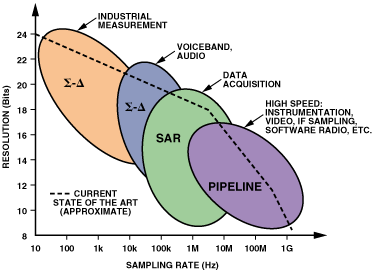
\includegraphics[scale=1]{ADC_Comp_Chart.png}
\caption{\textit{Chart displaying the classifications of different ADC architectures \cite{WaltKester:2005}}}
\label{fig:ADC_Comp_Chart}
\end{figure}
%
\subsubsection{Sampling Rate}		%EDIT THIS SECTION
\label{sec:adc_fin}
\indent The Nyquist-Shannon Sampling Criterion states that data must be sampled at a minimum of twice the expected frequencies being measured
\cite{MusaJouaneh:2013}. The accelerometer that was chosen for the preliminary lab experiments has a bandwidth of $500 Hz$, therefore the ADC must be able
to sample a minimum of $1kHz$. However, since frequencies expected from the lab testing are in the range of $0-60Hz$, the sampling frequency of the ADC
does not necessarily need to be so high. %Must reference source that states expected natural frequencies of bridges
%
\subsubsection{Power Consumption}
\label{sec:adc_power_cons.}
\indent Since the nature of this sensor package was to be a wireless sensor, it was assumed that all power used by the sensor package would be generated
using alternative energy. With this in mind, components used on board the sensor package have as little current draw as possible.
%
\subsubsection{Input Channels}
\label{sec:adc_in_ch_num}
\indent One important, but almost overlooked, characteristic of the ADC was the ability to support multiple input channels simultaneously. The ADC needed
to be able to read three channels from an accelerometer and at least two channels from a strain gauge. For prototyping purposes, it is typically difficult
to find ADC's with more than 4 inputs; most come in packages that require surface mount technology in order to use. It was decided to address this
problem by using multiple ADC's and interfacing them simultaneously on a serial communication bus. Subsection \ref{sec:adc_comm} discusses this in
further detail. It should also be noted that the inputs of the ADC will be configured for differential measurements. This gives the ability to compare
the sensor data to a noise reference, and thus make it possible to without the need to filter data. %Sentence on surface mounting is awkward.

%
\subsubsection{Communication}
\label{sec:adc_comm}
\indent As shown in Table \ref{tab:uProcOptions}, the BeagleBone Black supports multiple communication protocols, include but not limited to, SPI and
I$^{2}$C. The communication from the ADC to the main micro-controller was decided to be either  4-wire SPI or I$^{2}$C. The ADC will be the slave to the
micro-controller. A con using SPI as the communication method is that for each slave device in the communication loop, there must be a dedicated Slave
Select (SS) line. This puts a limitation on how many ADC's can be used in each sensor package. However, I$^{2}$C utilizes a central bus and 7 bit unique
addresses for slave selection.

\subsection{Analog-to-Digital Converter Selection}
\indent When searching for ADC's that fit the parameters set in Section \ref{sec:ADC_Parameters}, two devices were investigated; the TI ADS1211 and TI
ADS1115. Both devices are summarized in Table \ref{tab:ADC_Compare} and explained in detail below.

\begin{table}[H]
\begin{center}
\begin{tabular}{|p{2.5cm}| p{3cm} | p{3cm} |}
\hline
&\multicolumn{2}{c|}{\textbf{Analog-Digital Converter}}\\
\hline
\textbf{Parameter} & ADS1211 
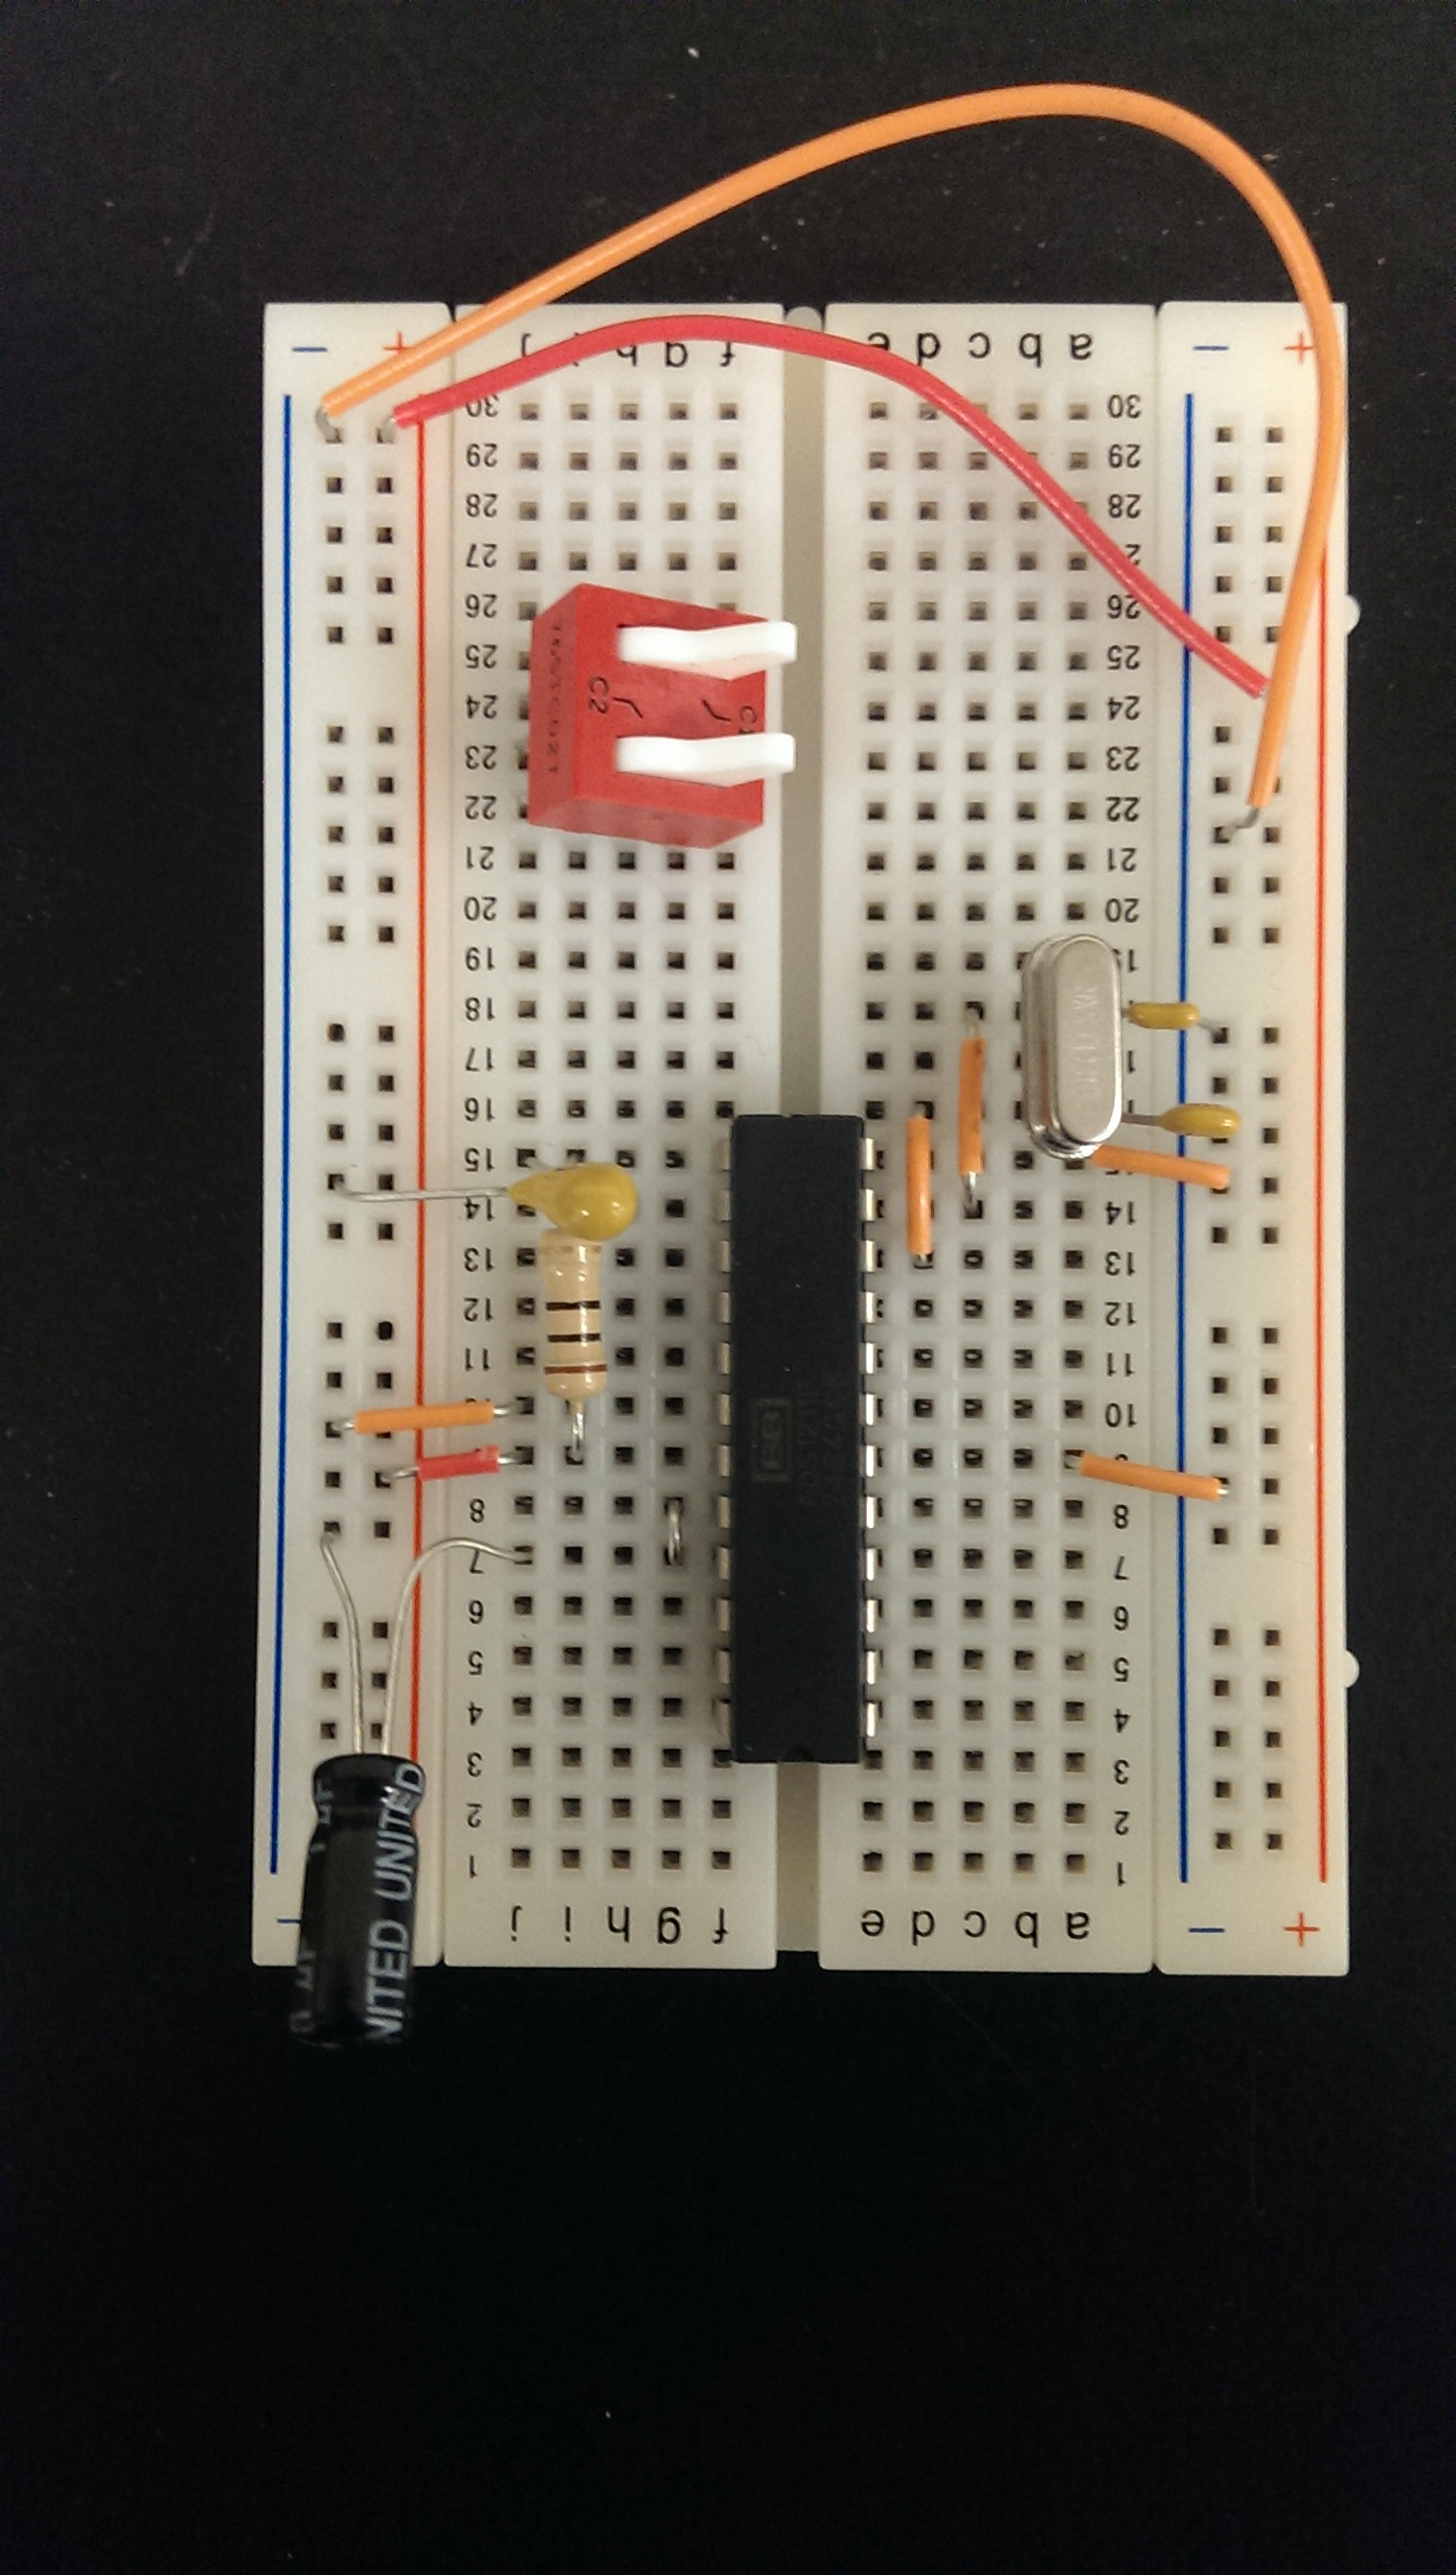
\includegraphics[width = 2.5cm]{oldadc}
& ADS1115
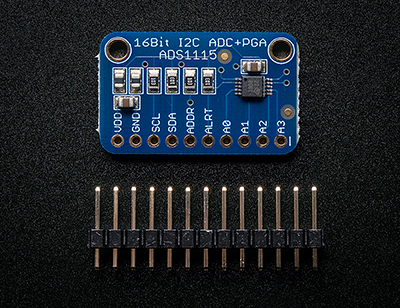
\includegraphics[width = 2.5cm]{ads1115}\\
\hline
Resolution: & 24 bits & 16 bits\\
\hline
Supported Communications:&	 SPI&I$^2$C\\
\hline
Power Consumption:&	5mW @ 5V	& 0.66 mW @ 3.3V\\
\hline

\end{tabular}
\caption{\textit{Comparison table of the ADS1211 and ADS1115 ADC devices}}
\label{tab:ADC_Compare}
\end{center}
\end{table}


\subsubsection{TI ADS1211}
\label{sec:ADC_ADS1211}
\indent The Texas Instruments ADS1211 24-Bit $\Delta \Sigma$ analog to digital converter features 20 effective bits of resolution at $1kHz$ under ideal
conditions; however that would be contingent upon the ability to design an ideal printed ciruit board (PCB) for the converter. Between 16 and 18 bits of
resolution are realistic for the initial prototype of the sensor package. By utilizing an internal 4-to-1 multiplexer, four input channels are available
to use. Recall that Section \ref{sec:adc_in_ch_num} requires at least five input channels, the ADS1211 falls short here. As a solution two ADC's would
be used, making it possible to read two strain gauges per sensor package as opposed to one. The ADS1211 datasheet provides information on synchronizing
multiple ADC's together. The converter draws approximately $10mA$ under typical working conditions. The converter utilizes the SPI protocol that is
supported by the BeagleBone Black.\\
\indent The ADS1211 was purchased and interfaced; however due to the complex circuitry that was required by the device, a month passed before the chip was
tested. The converter functioned correctly for approximately ten minutes and then stopped transmitting data. 
\subsubsection{TI ADS1115}
\label{sec:ADC_ADS1115}
\indent The Texas Instruments ADS1115 16-Bit analog to digital converter is of the same architecture as the ADS1211 ($\Delta \Sigma$). The chip also
features a multiplexer that allows up to 4 single ended or 2 differential inputs. The sampling frequency of the ADC is programmable from 8Hz to 860Hz, and
includes an internal oscillator. The average current draw for the ADS1115 is approximately $150\mu A$. There are two notable differences between the
ADS1115 and the ADS1211 ADCs. First, the ADS1115 communicates via the I$^{2}$C communication protocol. The ADS1115 has four unique I$^{2}$C addresses;
making it possible to have 16 single-ended inputs on one communication bus. Also, the chip was available pre-mounted on a PCB with all the necessary
supporting hardware; thus eliminating the possibility of incorrectly wiring up the circuit. 
\subsubsection{TI ADS1113}

\subsubsection{ADC Testing}
Preliminary lab tests were performed using a micro-controller with 12-bit ADC to collect data for analysis.
The time series that was returned did not accurately represent the data present, as verified with an oscilloscope.
It was determined that this was due to a difference in impedances between the accelerometer and the ADC.
The solution was to construct an op-amp circuit to match the impedances.
The ADS1115 has internal op-amps with programmable gain settings to avoid such issues.

\subsubsection{ADC Final Selection}
\indent Based on the comparison of the ADS1211 and the ADS1115 ADC's, the ADS1115 was chosen because of its ease of use and available Python libraries. 
